\chapter{ارزیابی}
در این بخش به تشریح نحوه‌ی ساخت مدلهای پیش‌بینی و ارزیابی معیارهای شرح داده شده در فصل \ref{chap:method} پرداخته می‌شود. با استفاده از معیارهای استخراج شده در فصل \ref{chap:case-study} مدلهای مورد نظر شاخته می‌شوند. ساخت مدل‌ها در زبان R انجام می‌گردد به وسیله‌ی بسته‌ی \نام{کرت}{Caret} \cite{kuhn2008caret} انجام می‌شود.\\
در ساخت و ارزیابی مدل‌ها از روش \واژه{ارزیابی میان دسته‌ای} استفاده می‌شود که تعداد دسته‌ها ۱۰ و تعداد تکرار نیز ۱۰ مورد می‌باشد. لازم به ذکر است که دسته‌بندی‌ها به طور تصادفی انجام می‌شود.  همچنین در بسته‌ی کرت در هر روش دسته‌بندی پارامترهای مختلفی به ور پیش فرض به کار گرفته می‌شود تا بهترین مدل ممکن ساخته شود. البته در این پژوهش همه‌ی مدل‌ها به منظور ارزیابی در نظر گرفته شده اند. به طور مثال در صورتی که در یک روش دسته‌بندی ۳ مقدار مختلف به عنوان پارامتر توسط بسته‌ی کرت انتخاب شود در کل ۳۰۰ مدل پیش بینی متمایز برای یک مجموعه از معیارها ساخته  خواهد شد. بدین ترتیب امکان تصادفی بودن پیش‌بینی‌ها نتایج به حداقل می‌رسد.\\
در ادامه هر یک از رویکردها به طور جداگانه ارزیابی می‌شوند.


\section{ارزیابی معیارهای فرآیند و جهش}
همانطور که اشاره شد هدف از این آزمایش این است که مشخص شود قرارگیری معیارهای جهش در کنار معیارهای فرآیند باعث بهبود پیش‌بینی خطا می‌گردد یا خیر و این تاثیر تا چه میزان است. به همین منظور یک با استفاده از ۱۲ معیار فرآیند دسته‌ای از مدل‌های پیش‌بینی ساخته شدند و دسته‌ی دیگر از مدل‌ها با استفاده از ۱۲ معیار فرآیند و ۴ معیار جهش ساخته شدند. در نهایت این دو دسته با استفاده از معیارهای ارزیابی مختلف با هم مقایسه شدند. بدیهی است که دو دسته‌ای که با هم مقایسه می‌شوند بجر در معیارهای استفاده شده (بردار ویژگی) به منظور ساخت مدل از هیچ منظری تفاوت ندارند. \\
در این ارزیابی از چهار روش دسته‌بندی استفاده شده است. این روش‌های دسته‌بندی بیش از سایرین در مقالات مورد استفاده قرار گرفته‌اند. لازم به ذکر است که این روش‌های دسته‌بندی را نمی‌توان با توجه به نتایج پیش‌بنی با هم مقایسه کرد. به عنوان مثال بالاتر بودن معیار صحت پیش‌بینی در یک روش از دیگر به الزاما معنی آن نیست که همواره این روش پیش‌بینی بر روی این مجموعه‌داده بهتر عمل می‌کند. زیرا در ساخت مدل‌ها در هر روش پارامترهای محتلفی استفاده شده و در نتیجه تعداد مدل‌های ساخته شده توسط هر روش دسته‌بندی متفات است.\\
در جدول \ref{tab:eval-phase1} بخشی از نتایج آمده است. این نتیاج نشان می‌دهد که قرار گیری معیارهای جهش در کنار معیارهای فرآیند موجب بهبود پیش‌بینی خطا به مقدار قابل ملاحظه‌ای می‌باشد. از میان روشهای دسته‌بندی بهترین عملکرد از نظر معیار صحت و دقت را روش \lr{Logestic Regression} داشته است. روش \lr{Neural Network } نیز بهترین عملکرد از نظر معیار بازخوانی را داشته است. همچنین بیشترین تغییر مثبت در صحت پیش‌بینی پس از افزودن معیارهای جهش را روش \lr{ Neural Network}  با مقدار $9.7$ درصد داشته است. همچنین کمترین تاثیر با مقدار $4.4$ درصد در روش Logestic Regression بوده است.
\begin{table}[H] 
	\renewcommand*{\arraystretch}{1.3}	
	\centering \caption{مقایسه‌ی معیارهای فرآیند به تنهایی  و به همراه جهش}
	\label{tab:eval-phase1}

	\begin{tabular}{|c|c|c|c|c|}
		
		\hline
		\hline
معیار & نام روش  & صحت & دقت & بازخوانی	
		\\
		\hline
		\hline
فرآیند & 
\lr{Decition Tree} & $0.627$&$0.669$&$0.492$
 \\
		\hline
		فرآیند و جهش & 
\lr{Decition Tree} & $0.707$&$0.710$&$0.692$
		\\
		\hline
فرآیند & 
\lr{SVM} & $0.648$&$0.665$&$0.587$
\\
\hline
فرآیند و جهش & 
\lr{SVM} & $0.703$&$0.716$&$0.665$
\\

\hline
فرآیند &
\lr{Logestic Regression} & $0.673$&$0.732$&$0.537$
\\
\hline
فرآیند و جهش & 
\lr{Logestic Regression} & $0.717$&$0.752$&$0.640$
\\
\hline
فرآیند &
\lr{Nueral Network} & $0.6092$&$0.628$&$0.517$
\\
\hline
فرآیند و جهش & 
\lr{Nueral Network} & $0.706$&$0.724$&$0.696$
\\
\hline		
	\end{tabular}
\end{table}

در شکل \ref{fig:ROC-phase1} نمودارهای ROC به تفکیک روش دسته‌بندی آمده است. در هر یک از زیر شکل‌ها منحنی ROC مربوط به  دو دسته با هم مقایسه شده است. در دسته‌ی اول مدل‌هایی که در ساخت آنها از معیارهای فرآیند استفاده شده  با خط ممتد نمایش داده شده است و دسته‌ی دوم مدل‌هایی هستند که از معیارهای فرآیند به همراه معیارهای جهش ساخته شده‌اند و با خط چین نمایش داده شده‌اند. همانطور که قابل مشاهده است در تمامی روش‌ها دسته‌بندی مدل‌های حاوی معیار جهش مساحت زیر نمودار بیشتری نسبت به دسته‌ی اول دارند و نشان از عملکرد این مدل‌ها می‌باشد. 
\begin{figure}[H]
	\begin{subfigure}{.5\textwidth}
		\centering
		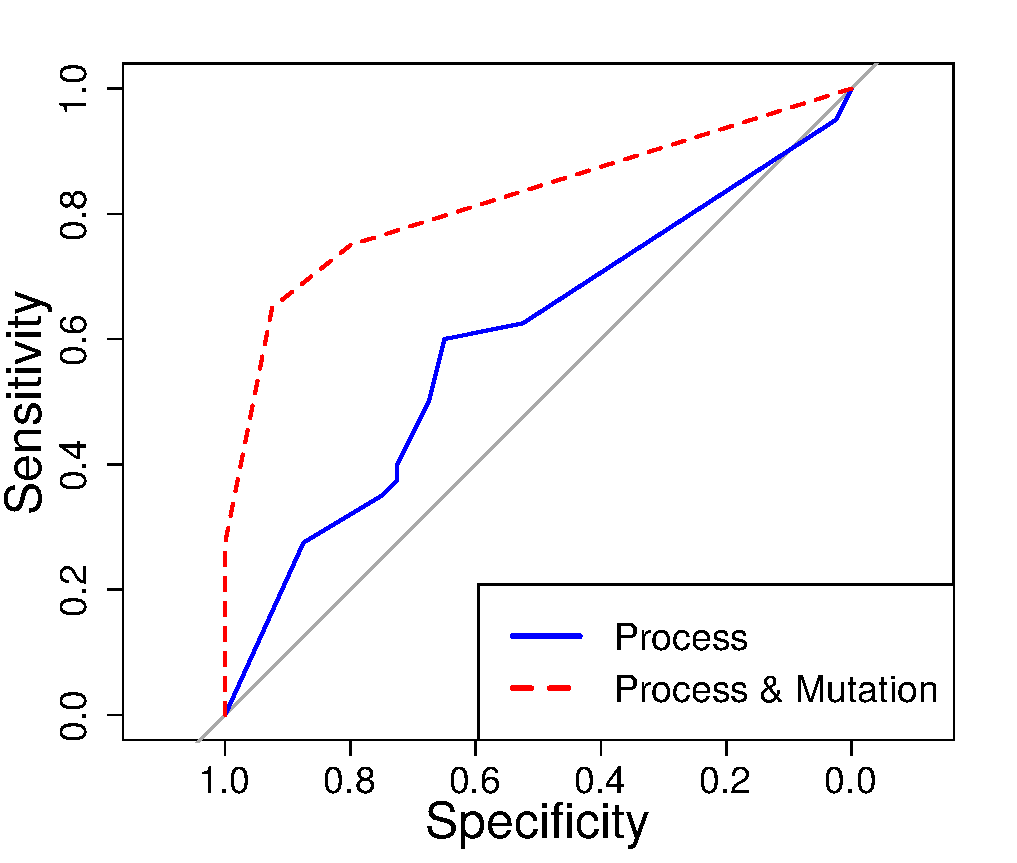
\includegraphics[width=\linewidth]{img/evaluation/phase1-roc-dt.pdf}
		\caption{\lr{Decition Tree}}
	\end{subfigure}
	\begin{subfigure}{.5\textwidth}
	\centering
	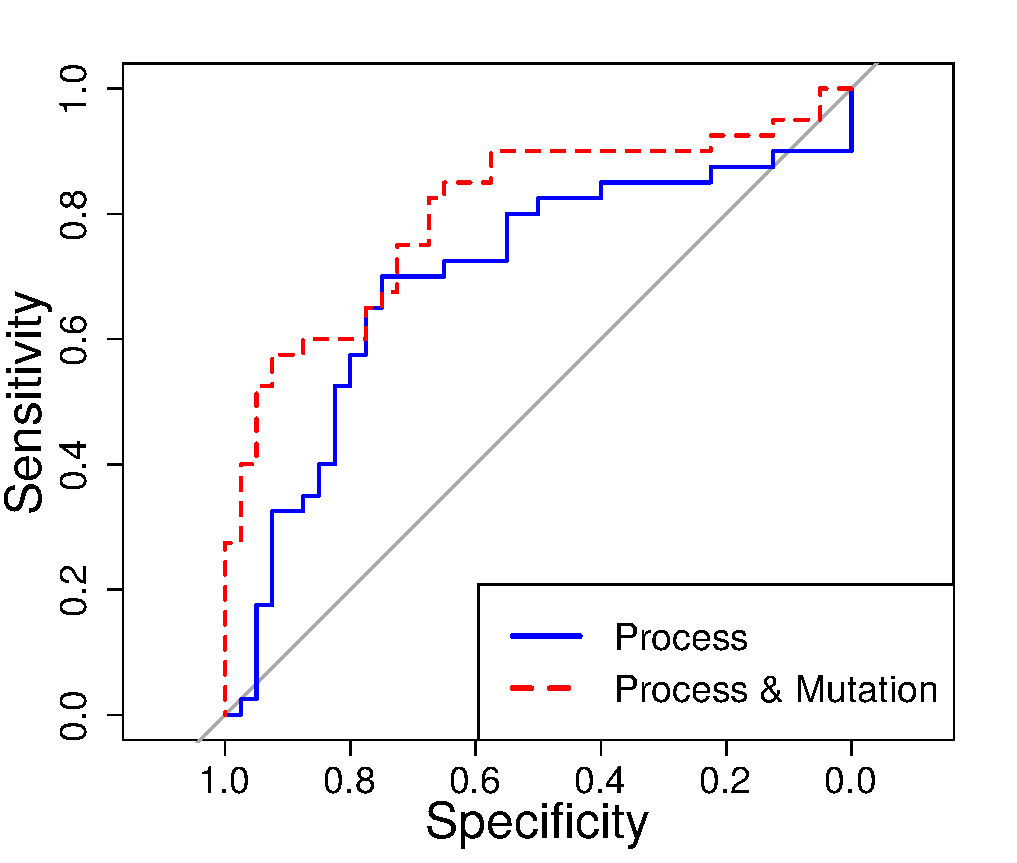
\includegraphics[width=\linewidth]{img/evaluation/phase1-roc-svm.pdf}
	\caption{SVM}
\end{subfigure}
	\begin{subfigure}{.5\textwidth}
	\centering
	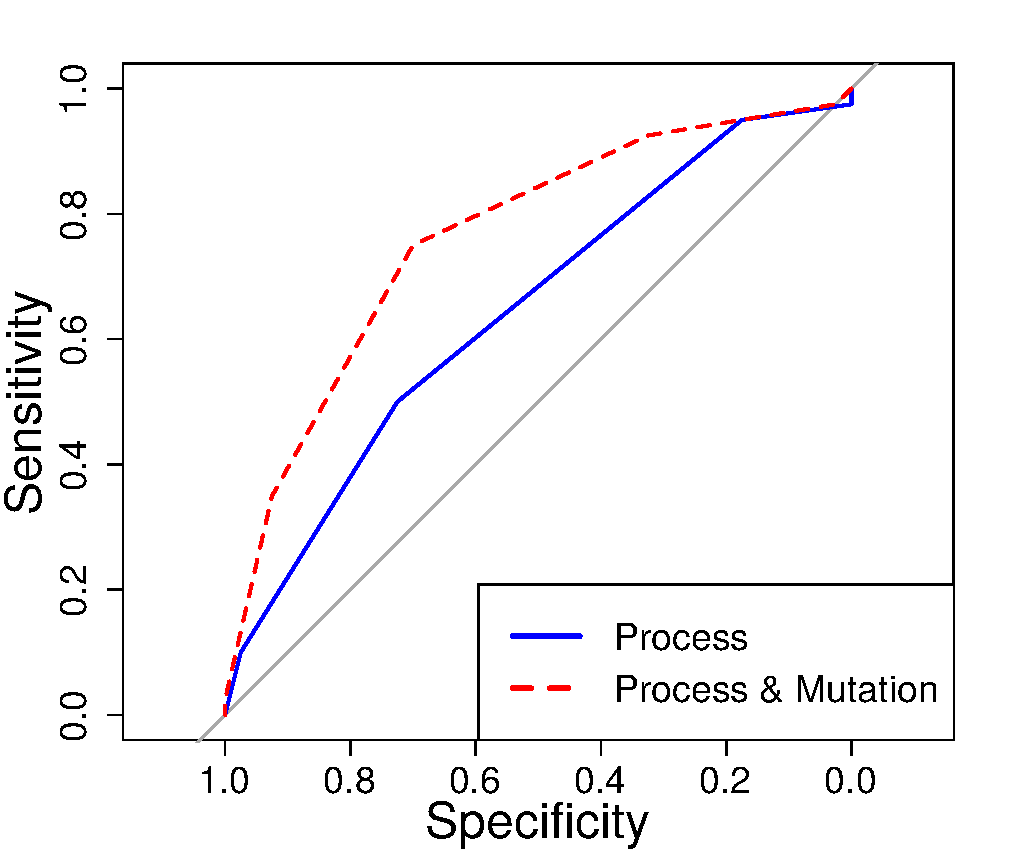
\includegraphics[width= \linewidth]{img/evaluation/phase1-roc-lr.pdf}
	\caption{\lr{Logestic Regression}}
\end{subfigure}
	\begin{subfigure}{.5\textwidth}
	\centering
	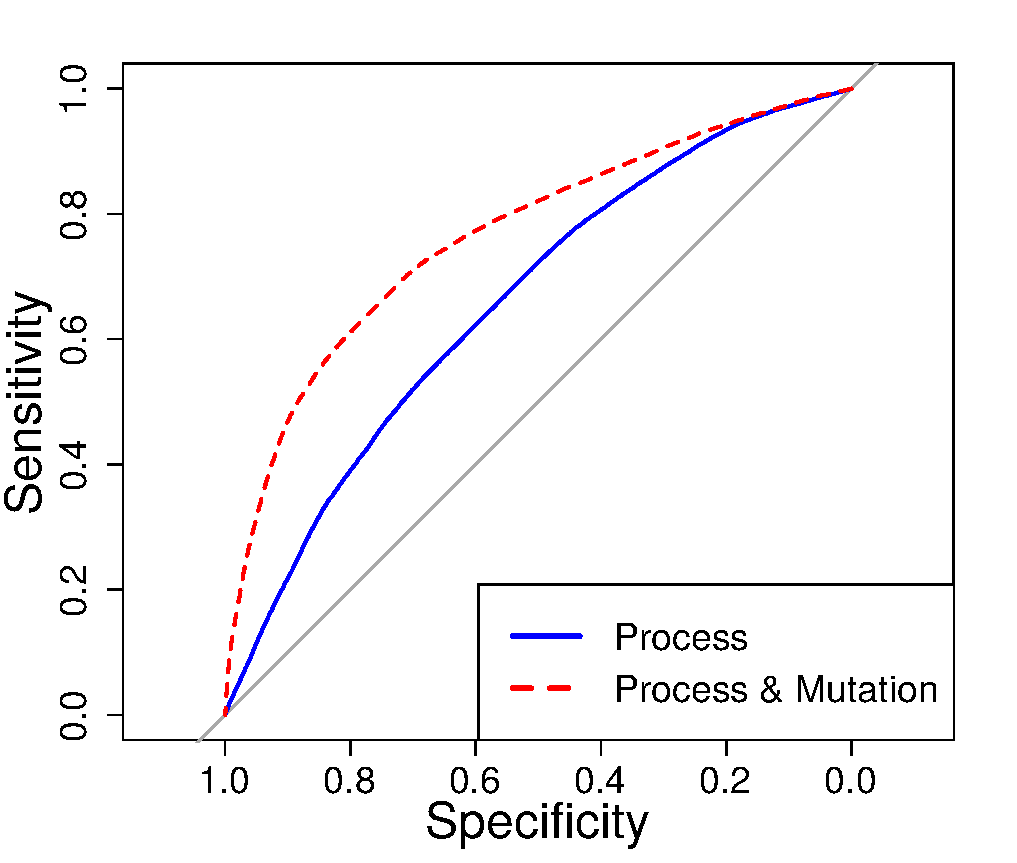
\includegraphics[width= \linewidth]{img/evaluation/phase1-roc-nn.pdf}
	\caption{\lr{Nueral Network}}
\end{subfigure}
\caption{نمودارهای ROC معیارهای فرآیند و به همراه جهش}
\label{fig:ROC-phase1}
\end{figure}

در جدول \ref{tab:auc-phase1} مساحت زیر نمودار ROC در هر یک از روش‌های دسته‌بندی آورده شده است. این جدول نشان می‌دهد بیشترین مقدار مساحت زیر نمودار در روش Logestic Regression بدست آمده است و کمترین مساحت متعلق به روش Decition Tree است. همچنین بیشترین تغییر مثبت با مقدار $11.1$ درصد به روش Neural Network تعلق دارد. همچنین لازم به ذکر است که کمترین مقدار مساحت با استفاده از معیارهای جهش و فرآیند از بیشترین مقدار مساحت با استفاده از معیارهای فرآیند به تنهایی بیشتر است. این موضوع نشان از تاثیر قابل توجه معیارهای جهش می‌باشد. 

\begin{table}[H] 
	\renewcommand*{\arraystretch}{1.2}	
	\centering \caption{مقادیر زیر نمودار ROC معیارهای فرآیند و به همراه جهش}
	\label{tab:auc-phase1}
	\begin{tabular}{|c|c|c|c|c|}
		\hline
		\hline
		معیار & 
		 \lr{ Decition Tree} & SVM &\lr{ Logestic Regression} &\lr{ Neural Network} \\
		 \hline
		 \hline
		 فرآیند & $.666$ & $.696$ & $.721$ & $.654$
		 \\
		 \hline
		 فرآیند و جهش  & $.745$ & $.782$ & $.792$ & $.765$
		 \\
		 \hline
		 
	\end{tabular}
\end{table}

\section{ارزیابی فرآیند مبتنی بر جهش }
